\documentclass[a4paper, 10pt]{article}
\hyphenpenalty=8000
\textwidth=125mm
\textheight=185mm

\usepackage{graphicx}
%this package is flexible for image insertion
%
\usepackage{alltt}
%this package is suitable for the description of algorithms and computer programs
%
\usepackage{amsmath}
%this package draws mathematical symbols smoothly
%
\usepackage[hidelinks, pdftex]{hyperref}
%this package produces hypertext links in the document

\pagenumbering{arabic}
\setcounter{page}{1}
\renewcommand{\thefootnote}{\fnsymbol{footnote}}
\newcommand{\doi}[1]{\href{https://doi.org/#1}{\texttt{https://doi.org/#1}}}

\begin{document}

\begin{center}
Nonlinear Analysis: Modelling and Control, Vol. vv, No. nn, 2025\\
\copyright\ Vilnius University\\[24pt]
\LARGE
\textbf{Operaciones Vectoriales}\footnote{This research was supported by grant No.\ xxxx.}\\[6pt]
\small
\textbf{Diego Alzate, Aris Avila, Julieth Gutierrez}\\[6pt]
Ie Infotep of author(s), address(es) \\[6pt]
Received: date\quad/\quad
Revised: date\quad/\quad
Published online: date
\end{center}

\begin{abstract}
Este informe presenta una simulación de movimiento y rotación de vectores en un plano cartesiano. Se desplaza un punto (vector) dentro de un área rectangular y se aplica una rotación a dicho vector. Los resultados muestran cómo el desplazamiento y la rotación afectan las coordenadas del vector, con visualizaciones claras de los vectores antes y después de la rotación. \texttt). \vskip 2mm

\textbf{Keywords:} Vectores, rotación, simulación.
\end{abstract}

\nocite{2009ProcDETAp}

\section{Introducción}\label{s:1}
En este proyecto, se implementa una simulación para ilustrar cómo se desplaza y rota un vector en el plano cartesiano. El objetivo principal es entender y visualizar los efectos del desplazamiento y la rotación de vectores. A través de la simulación, los resultados muestran cómo el vector cambia en sus coordenadas debido a estas operaciones. En este informe se describen las fórmulas matemáticas utilizadas para llevar a cabo estas operaciones.

\section{Operaciones Vectoriales}\label{s:2}
A continuación se detallan las fórmulas matemáticas utilizadas en este trabajo para realizar las operaciones sobre vectores: desplazamiento, producto interno, norma vectorial y rotación.

\subsection{Operador Vectorial Escalar}\label{s:2.1}
El **producto escalar** o **producto interno** entre dos vectores \( \mathbf{a} = [a_1, a_2] \) y \( \mathbf{b} = [b_1, b_2] \) se define como:
\[
\mathbf{a} \cdot \mathbf{b} = a_1 \cdot b_1 + a_2 \cdot b_2
\]
Este producto escalar devuelve un número real (escalar) y tiene aplicaciones en física, geometría y álgebra lineal.

\subsection{Norma Vectorial}\label{s:2.2}
La norma o magnitud de un vector \( \mathbf{v} = [v_1, v_2] \) se calcula como la raíz cuadrada de la suma de los cuadrados de sus componentes:
\[
||\mathbf{v}|| = \sqrt{v_1^2 + v_2^2}
\]
Este cálculo proporciona la longitud del vector y es fundamental para medir la distancia en el espacio.

\subsection{Rotación de un Vector}\label{s:2.3}
La rotación de un vector \( \mathbf{v} = [v_1, v_2] \) en el plano 2D por un ángulo \( \theta \) se realiza mediante la matriz de rotación:
\[
R(\theta) = \begin{bmatrix} \cos(\theta) & -\sin(\theta) \\ \sin(\theta) & \cos(\theta) \end{bmatrix}
\]
La rotación del vector \( \mathbf{v} \) es el resultado de multiplicar la matriz de rotación por el vector:
\[
\mathbf{v'} = R(\theta) \cdot \mathbf{v}
\]
El vector rotado \( \mathbf{v'} \) es el nuevo vector después de aplicar la rotación.

\section{Descripción de la Actividad}\label{s:3}
En este proyecto, se desarrolló una simulación utilizando Python para ilustrar las operaciones de desplazamiento y rotación de un vector. La clase `Simulacion` se encarga de realizar los cálculos y visualizar los resultados. El punto inicial del vector se define en un plano cartesiano de tamaño fijo \( 10 \times 10 \) unidades. Se implementaron los siguientes métodos:
- Desplazamiento: El vector se mueve a lo largo de una dirección (derecha, izquierda, arriba, abajo).
- Rotación: El vector se rota alrededor del origen por un ángulo especificado.

La visualización de los resultados se realiza a través de gráficos donde se muestran tanto el vector original como el vector rotado.

\section{Resultados}\label{s:4}
Los resultados de la simulación mostraron cómo el vector cambia cuando se le aplica un desplazamiento y una rotación. Por ejemplo, cuando el vector se desplaza 2 unidades a la derecha, su posición cambia de \( (5, 5) \) a \( (7, 5) \). Posteriormente, al aplicar una rotación de 45 grados, el vector rotado se desplaza a una nueva posición, lo que ilustra claramente el efecto de la rotación sobre el vector en el plano cartesiano.

A continuación, se presenta una imagen que muestra el vector original y el vector rotado después de ser desplazado:

\begin{figure}[h!]
    \centering
    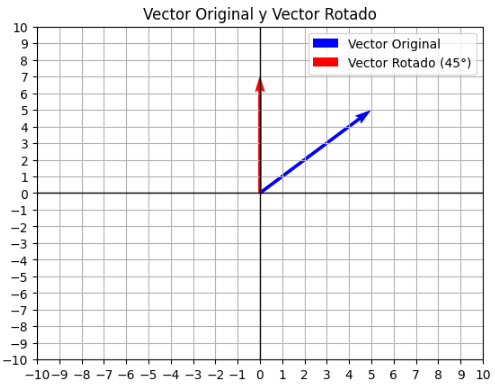
\includegraphics[width=0.6\textwidth]{resultado.png}
    \caption{Vector original y vector rotado después de un desplazamiento de 2 unidades hacia la derecha y una rotación de 45 grados.}
    \label{fig:resultados}
\end{figure}

\section{Conclusión}\label{s:5}
Este proyecto permite visualizar y entender cómo las operaciones de desplazamiento y rotación afectan a un vector en el plano cartesiano. La implementación de la simulación proporcionó una herramienta útil para estudiar estos conceptos, y la visualización gráfica facilitó la comprensión de los cambios en las coordenadas del vector. Se recomienda continuar ampliando la simulación para incluir más operaciones vectoriales, como la reflexión y las transformaciones lineales.

\end{document}